\documentclass{beamer}
%
% Choose how your presentation looks.
%
% For more themes, color themes and font themes, see:
% http://deic.uab.es/~iblanes/beamer_gallery/index_by_theme.html
%
\mode<presentation>
{
  \definecolor{StanfordCardinal}{RGB}{140, 21, 21} % Stanford Cardinal (primary)
  \usetheme{Madrid}      % or try Darmstadt, Madrid, Warsaw, ...
  \usecolortheme[named=StanfordCardinal]{structure} % or try albatross, beaver, crane, ...
  \usefonttheme{default}  % or try serif, structurebold, ...
  \setbeamertemplate{navigation symbols}{}
  \setbeamertemplate{caption}[numbered]
  %\useinnertheme{circles}
  %\useoutertheme{miniframes} % Alternatively: miniframes, infolines, split
} 
\usepackage{xcolor}
\usepackage[english]{babel}
\usepackage[utf8x]{inputenc}

\title[NN Workshop]{Introduction to Neural Networks}
\author{Klint Kanopka}
\institute{kkanopka@stanford.edu}
\date{Wednesday, May 15, 2019}

\begin{document}

    \begin{frame}
      \titlepage
    \end{frame}
    
    \begin{frame}{Outline}
      \tableofcontents
    \end{frame}
    
    \section{Introduction}
    
        \subsection{Logistic Regression}
            \begin{frame}{Logistic Regression}
                \begin{itemize}
                    \item<2-> Computer scientists call the logistic function the ``sigmoid''
                    $$ \sigma(x)= \frac{1}{1+e^{-x}} $$
                    \item<3-> Maps inputs to real numbers on the interval $(0,1)$
                    \item<4-> Good for turning numbers into probabilities
                    \item<5-> Has a really simple derivative:
                    $$ \frac{d\sigma}{dx} = \sigma(x)(1-\sigma(x)) $$
                    \item<6-> This is super useful for neural nets, as we'll discuss later.
                \end{itemize}
            \end{frame}
        \subsection{Maximum Likelihood Estimation}
            \begin{frame}{Maximum Likelihood Estimation}
                \begin{itemize}
                    \item<2-> Models use parameters to relate data within observations
                    \item<3-> MLE specifies a likelihood function that describes how likely (probable) it is to observe the data we have, given a set of model parameters
                    \item<4-> MLE searches for model parameters that maximize the likelihood function
                    \item<5-> Often work in terms of log likelihood
                \end{itemize}
            \end{frame}
        
        \subsection{Motivations for Neural Networks}

            \begin{frame}{Machine Learning}
                \begin{itemize}
                    \item<2-> Subfield of Artificial Intelligence
                    \item<3-> Computers ``learn'' models from data
                    \begin{itemize}
                        \item <4-> Instead of specifying a strict functional form (linear, logistic, etc.) and doing a regression, the computer learns the shape of the function and its parameters from the data
                        \item<5-> The data the computer learns from is called the ``training set''
                    \end{itemize}
                    \item<6-> Works great for prediction and classification tasks
                    \item<7-> Less useful for inference (and causal inference), but this is changing
                \end{itemize}
            \end{frame}
            
            \begin{frame}{Why Neural Nets?}
                \begin{itemize}
                    \item<2-> We have tons of data
                    \item<2-> Compute time is getting increasingly cheap
                    \item<3-> The quality of an estimate is highly dependent on model specification
                    \item<4-> More flexible estimation techniques allow computers to learn functional forms
                    \item<5-> Neural networks are ``universal approximators'' and can learn arbitrarily complex  functional forms
                \end{itemize}
            \end{frame}
            
    \section{Structure and Design}    
    
        \begin{frame}{Guiding Idea}
            \begin{itemize}
                \item<2-> Neural networks are built out of \em nodes.\em
                \item<3-> These nodes are organized into \em hidden layers.\em
                \item<4-> For now, each node consists of an individual sigmoid function (logistic regression)
                \item<5-> \em Examples on the board... \em
            \end{itemize}
        \end{frame}
        
    \section{Estimation and Application}
    
        \begin{frame}{Training/Test Data}
            \begin{itemize}
                \item<2-> Conventional wisdom says to split your data 80/20 into training/test data
                \item<3-> This is often terrible advice
                \item<4-> The purpose of this is to hold out some data to test how well your model generalizes
                \item<5-> If you only have a little bit of data, this will work. If you have more, use a \em dev set.\em
                \item<6-> The dev set helps you tune \em hyperparameters \em like number of nodes, number of hidden layers, and learning rate
                \item<7-> Good splits (train/dev/test) are 80/10/10, 90/5/5, or even 98/1/1 if you have a ton of data
                \item<8-> More training data translates into a more robust model
            \end{itemize}
        \end{frame}
        
        \begin{frame}{Loss Functions}
            \begin{itemize}
                \item<2-> A function that defines how wrong your current predictions are
                \item<3-> For binary classification (1 or 0):
                $$ L = -\sum_{i=1}^N y_i \log\hat{y}_i + (1 - y_i) \log (1-\hat{y}_i) $$
                \item<4-> For continuous variables:
                $$ L = \sum_{i=1}^N (y_i - \hat{y}_i)^2 $$
                \item<5-> General goal: Minimize how wrong you are
            \end{itemize}
        \end{frame}
        
        \begin{frame}{Estimation}
            \begin{itemize}
                \item Estimation is done with an algorithm called \em backpropagation \em
                \item Similar to MLE, except now we search over parameters to \em minimize \em the loss function
                \item Updates to the individual parameters in the model are typically done via \em gradient descent \em
                \item Similar to Newton-Raphson, but doesn't require inverting a Hessian and requires more iterations to converge - in big data applications, often faster (smaller but quicker steps)
            \end{itemize}
        \end{frame}
        
        \begin{frame}{Application}
            \begin{center}
                Clone or download the files from the github repo:\\
                \vskip 1cm
                https://github.com/klintkanopka/nn\_workshop
            \end{center}
        \end{frame}
        
    \section{Other Neural Architectures}
    
            \begin{frame}{Feed-Forward Neural Networks}
                \begin{figure}
                    \centering
                    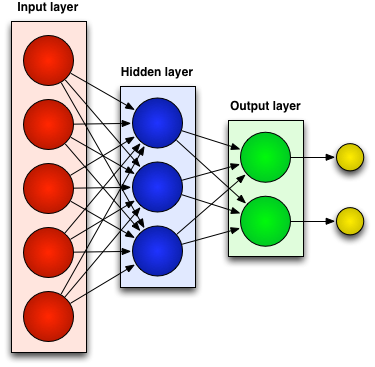
\includegraphics[scale=0.45]{nn-feedforward.png}
                    \caption{Feed-Forward Neural Network. Image Credit: Joseph Wilk}
                \end{figure}
            \end{frame}
    
        \subsection{Recurrent Neural Networks}
        
            \begin{frame}{Recurrent Neural Networks}
                \begin{itemize}
                    \item<2-> Operate on series or sequence of data
                    \item<3-> The same network is applied at each time step
                    \item<4-> Each time step also takes the output of the previous time step as input
                    \item<5-> Specialized versions of the RNN work to help ``remember'' older data:
                    \begin{itemize}
                        \item<6-> Gated Recurrent Unit (GRU)
                        \item<7-> Long Short Term Memory (LSTM)
                    \end{itemize}
                \end{itemize}
            \end{frame}
      
            \begin{frame}{Recurrent Neural Networks}
                \begin{figure}
                    \centering
                    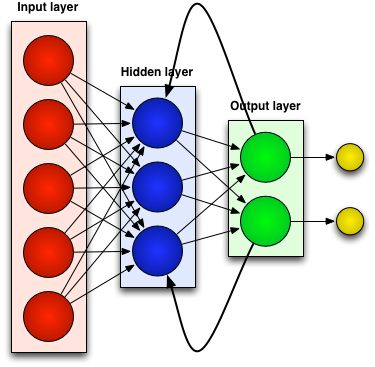
\includegraphics[scale=0.45]{nn-recurrent.png}
                    \caption{Recurrent Neural Network. Image Credit: Joseph Wilk}
                \end{figure}           
            \end{frame}
            
            \begin{frame}{Recurrent Neural Networks}
                Useful for:
                \begin{itemize}
                    \item<2-> Sequences of data
                    \item<3-> Item responses
                    \item<4-> Text
                    \item<5-> Time series data
                    \item<6-> Panel data
                \end{itemize}
            \end{frame}
            
        \subsection{Convolutional Neural Network}   
            
            \begin{frame}{Convolutional Neural Networks}
                \begin{itemize}
                    \item<2-> Uses a window (or kernel) to perform arithmetic reductions on subsets of the input
                    \item<3-> These windows are called filters and can learn to detect features in the input
                \end{itemize}
            \end{frame}
                    
            \begin{frame}{Convolutional Neural Networks}
                \begin{figure}
                    \centering
                    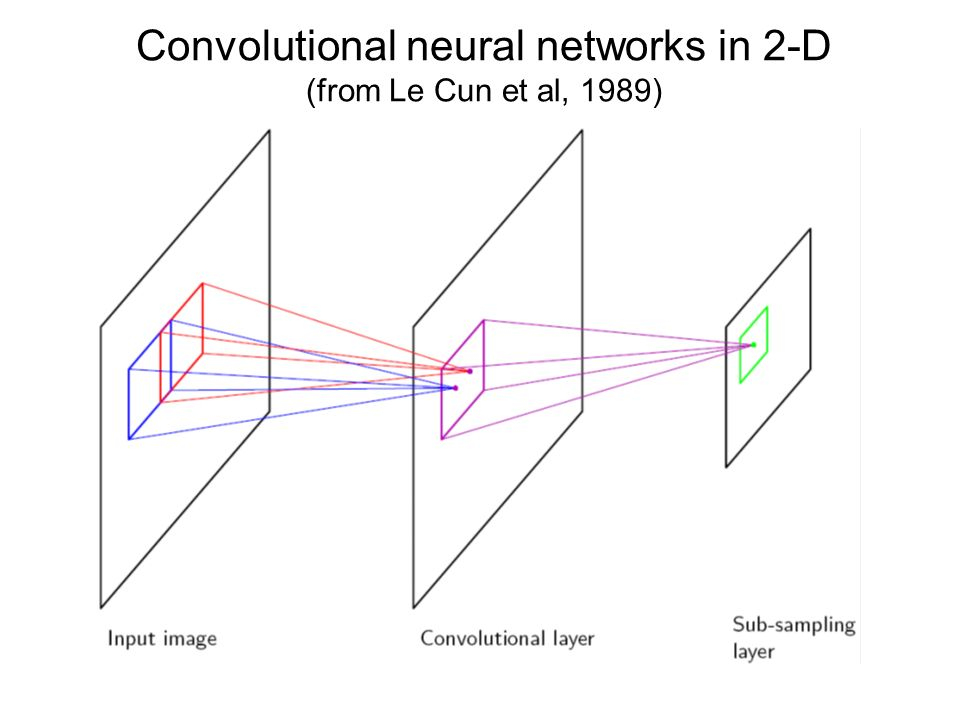
\includegraphics[scale=0.35]{nn-conv.jpg}
                \end{figure}                 
            \end{frame}
            
            \begin{frame}{Convolutional Neural Networks}
                Useful for:
                \begin{itemize}
                    \item<2-> Arrays of data
                    \item<3-> Images
                    \item<4-> Sequences of data
                    \item<5-> Text
                    \item<6-> Signal processing
                \end{itemize}
            \end{frame}
        
        \subsection{Deep Learning}
        
            \begin{frame}{Deep Learning}
                \begin{itemize}
                    \item<2-> Tech bro buzzword for large neural networks
                    \item<3-> "Deep" refers lots of hidden layers
                    \item<4-> Leverages huge amounts of data
                    \item<5-> Trained/run on cloud servers with GPUs/TPUs
                    \item<6-> Good word to stick into things you want to get published or funded
                \end{itemize}                 
            \end{frame}
        
  
    \begin{frame}{I'm Done}
        \begin{center}
            Thank you for your attention. \\
            \vskip 1cm
            Klint Kanopka \\
            kkanopka@stanford.edu\\
            \vskip 1cm
            To download today's materials:\\
            https://github.com/klintkanopka/nn\_workshop
        \end{center}
    \end{frame}
    
\end{document}
